\subsubsection{Algoritmo de detección de cintas}

El algoritmo de detección explota el alto contraste entre la cinta negra y el fondo claro mediante procesamiento en el canal V del espacio HSV, aprovechando su invariancia ante cambios cromáticos de iluminación.\\

El proceso consta de tres etapas:\\

\underline{Etapa 1 - Conversión a HSV:} La imagen RGB capturada se transforma al espacio HSV y se extrae el canal V que representa el brillo de cada píxel.\\

\underline{Etapa 2 - Umbralización inversa:} Sobre el canal V se aplica umbralización inversa con umbral 50:

\begin{equation}
I_{bin}(x,y) = \begin{cases}
255 & \text{si } I_V(x,y) < 50 \\
0 & \text{si } I_V(x,y) \geq 50
\end{cases}
\end{equation}

\underline{Etapa 3 - Detección de contornos:} Se ejecuta el algoritmo de Suzuki-Abe sobre la imagen binaria, filtrando contornos con área mínima de 500 píxeles para eliminar ruido y sombras.

\subsubsection{Evaluación de calidad del contorno}

Los contornos que superan el filtrado de área se evalúan para discriminar cintas genuinas de otros elementos oscuros (plantas, vasos). La evaluación analiza la región basal, definida como el 10\% inferior del delimitador del contorno.

Para cada contorno se calcula la fracción de píxeles blancos en su región basal:

\begin{equation}
Q_{base} = \frac{1}{|R_{base}|} \sum_{(x,y) \in R_{base}} \frac{I_{bin}(x,y)}{255}
\end{equation}

Un valor $Q_{base}$ cercano a 1 indica una región basal consistentemente oscura con borde inferior nítido, característico de las cintas. Las cintas genuinas presentan $Q_{base} > 0.8$, mientras que plantas u otros objetos tienen $Q_{base} < 0.5$. Se establece un umbral de aceptación de 0.7.

\subsubsection{Sistema de evaluación ponderada}

Cuando múltiples contornos cumplen los criterios de área y calidad basal, se selecciona el mejor candidato mediante evaluación ponderada que combina tres factores:

\begin{itemize}
    \item \underline{Área normalizada} ($S_{área}$): Favorece áreas intermedias entre 500 y 50000 píxeles, descartando ruido o elementos excesivamente grandes.

    \item \underline{Posición del centroide} ($S_{posición}$): Favorece contornos cercanos al centro de la imagen, asumiendo que el robot se posiciona frente a la cinta objetivo.

    \item \underline{Calidad basal} ($Q_{base}$): Favorece contornos con bordes inferiores nítidos.
\end{itemize}

La puntuación total se calcula como:

\begin{equation}
P_{total} = w_1 \cdot S_{área} + w_2 \cdot S_{posición} + w_3 \cdot Q_{base}
\end{equation}

con pesos $w_1 = 0.3$, $w_2 = 0.4$ y $w_3 = 0.3$, otorgando mayor importancia a la posición. El contorno con mayor puntuación se selecciona como cinta de referencia.

\begin{figure}[H]
\centering
\begin{subfigure}[b]{0.48\textwidth}
    \centering
    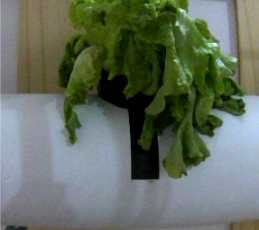
\includegraphics[width=0.7\textwidth]{imagenes/detector_marcadores_1_original.png}
    \caption{Imagen RGB original capturada}
\end{subfigure}
\hfill
\begin{subfigure}[b]{0.48\textwidth}
    \centering
    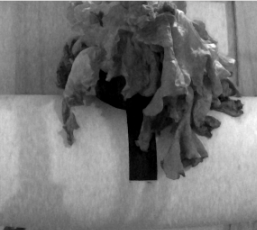
\includegraphics[width=0.7\textwidth]{imagenes/detector_marcadores_2_canal_v.png}
    \caption{Canal V extraído (brillo)}
\end{subfigure}

\vspace{0.3cm}

\begin{subfigure}[b]{0.48\textwidth}
    \centering
    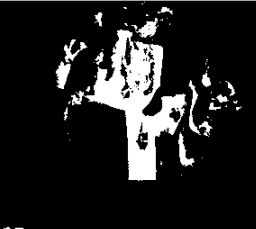
\includegraphics[width=0.7\textwidth]{imagenes/detector_marcadores_3_binario.png}
    \caption{Umbralización binaria inversa (T=50)}
\end{subfigure}
\hfill
\begin{subfigure}[b]{0.48\textwidth}
    \centering
    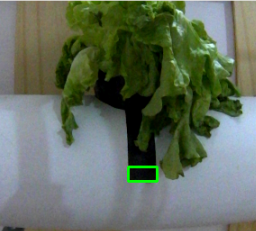
\includegraphics[width=0.7\textwidth]{imagenes/detector_marcadores_4_contornos.png}
    \caption{Contornos detectados con evaluación ponderada}
\end{subfigure}

\caption{\textit{Secuencia de procesamiento del detector de cintas mostrando las transformaciones sucesivas de la imagen}}
\label{fig:proceso_marcadores}
\end{figure}

\subsubsection{Métricas de desempeño}

Evaluado sobre 35 frames de barrido horizontal (20 con cintas, 15 sin cintas):

\begin{table}[H]
\centering
\begin{tabular}{|l|r|}
\hline
\textbf{Métrica} & \textbf{Valor} \\ \hline
Sensibilidad (Recall) & 90.0\% (18/20) \\ \hline
Especificidad & 100\% (15/15) \\ \hline
Precisión (Precision) & 100\% (18/18) \\ \hline
Error de localización X medio & 3.2 mm \\ \hline
Error máximo de localización X & 8.7 mm \\ \hline
\end{tabular}
\caption{Desempeño del detector de cintas}
\label{tab:metricas_cintas}
\end{table}

Matriz de detección para cintas:

\begin{table}[H]
\centering
\begin{tabular}{cc|c|c|}
\cline{3-4}
& & \multicolumn{2}{c|}{\textbf{Predicción}} \\ \cline{3-4}
& & Cinta detectada & No cinta \\ \hline
\multicolumn{1}{|c|}{\multirow{2}{*}{\textbf{Real}}} & Cinta & 18 & 2 \\ \cline{2-4}
\multicolumn{1}{|c|}{} & No cinta & 0 & 15 \\ \hline
\end{tabular}
\caption{Matriz de detección binaria - cintas}
\label{tab:confusion_cintas}
\end{table}

\noindent
Los 2 falsos negativos se debieron a cambios en la incidencia de la iluminación sobre las cintas lo que que redujo el contraste entre cinta y fondo.
